\chapter{Design \& Implementation}\label{chap:design}
In this chapter we will introduce our final idea, which is ultimately our solution. We explain the system top-down, and as such we broadly describe the entire system before diving into the specifics.

\begin{chapterorganization}
  \item In \sectionref{sec:design_overview} we provide an introductory overview of the system architecture and explain how the components interact;
  \item In \sectionref{sec:database} we argue for and choose a database to store a Wikipedia data structure;
  \item In \sectionref{sec:data} we explain the data sources, how we process the data, and how we insert the data into the chosen database;
  \item In \sectionref{sec:detailed_view} we describe components of the system in greater detail. \todo{more text describing this};
  \item In \sectionref{sec:design_ui} we present the design of a user interface for the system.
\end{chapterorganization}

\section{Overview}\label{sec:design_overview}
The purpose of the system is to suggest link suggestions for articles, and add these to a pool of suggestions. A user can then browse this pool for suggestions of articles to improve the outgoing links.

The system consists of a pipeline utilizing two trained models in order to make predictions. These models are
\begin{enumerate*}[label=(\roman*)]
  \item a feature extraction model, and
  \item a classifier model.
\end{enumerate*}
Both of these models are trained by temporally separate workflows. A diagram of the main pipeline and the separate workflows for training the models can be seen in \cref{fig:system-overview}. In the following sections, the main areas will be explained.

\tikzsetnextfilename{system-overview}
\begin{figure}[tbp]%
  \centering
  \begin{tikzpicture}[node distance = 2.84cm, auto]
    \node [database, yshift=1em] (db) {DB};
    \node [bigblock, right of=db] (ap) {Article Picker};
    \node [bigblock, right of=ap] (tfl) {Feature Extraction};
    \node [bigblock, right of=tfl] (classifier) {Classifier};
    \node [database, right of=classifier] (db2) {DB2};
    \node [bigblock, below=1cm of db2] (web) {Web Interface};
    
    %\node [above=1cm of ap] (inputarticle) {};
    
    \node [smallblock, below=1.5cm of ap, xshift=-2em] (n2v) {Node2Vec};
    \node [smallblock, below=.5cm of n2v] (paropt) {Parameter Optimizer};
    
    \node [smallblock, below=4.5cm of tfl] (prepper) {Training Data Generator};
    \node [smallblock, right of=prepper] (classifierTrainer) {Classifier Trainer};
    
    \begin{scope}[on background layer]
    \node [container, fit=(n2v)(paropt)] (container1) {};
    \node[below] at (container1.north) {Feature Learning};
    \node [container, fit=(prepper)(classifierTrainer)] (container2) {};
    \node[above] at (container2.south) {Classifier Model Learning};
    
    \node [container, fit=(db)(db2)] (container3) {};
    \node[below] at (container3.north) {Main Pipeline};
    \end{scope}
    
    %\draw [->] (db) -- (n2v);
    
    \path [line] (db) -- (ap);
    %\path [line] (inputarticle) -- (ap);
    \path [line] (ap) -- (tfl);
    \path [line] (tfl) -- (classifier);
    \path [line] (classifier) -- (db2);
    \path [line] (db2) -- (web);
    
    \path [line] (db.300) |- (n2v);
    %\path [line] (db.300) |- (paropt);
    \path [line] (db.240) |- (prepper);
    
    \path [line, swap, transform canvas={xshift=-1.3em}] (paropt) -- node{Parameters} (n2v);
    \path [line] (n2v.east) -| node [near end] {Model} ([xshift=-1.2em]tfl.south);
    
    \path [line] (prepper) -- (classifierTrainer);
    %\path [line] (prepper) -- (tfl);
    %\path [line] ([xshift=1.2em]tfl.south) -- ([xshift=1.2em]prepper.north);
    \draw [line] (prepper.north) |- ([xshift=1.2em, yshift=0.5em]tfl.south) -- ([xshift=1.2em]prepper.north);
    
    \path [line] (classifierTrainer) -- node{Model} (classifier);
    
  \end{tikzpicture}
\caption[Architecture diagram showing the major components of the system]{Architecture diagram showing the major components of the system. Each box is a component, and a dashed line box is a grouping of components. Arrows describe the way data flows.}%
\label{fig:system-overview}%
\end{figure}

%Throughout this chapter the different components will be explained in detail.


\subsection{Main Pipeline}
The main part of the system provides link suggestions for articles. Because it is computationally intensive to check if each of the 5.2 million articles should link to each other, we split the pipeline into a \emph{filtering} and a \emph{refinement} step. The filtering step filter out some obvious bad candidates based on some heuristic. The refinement step consists of a trained classifier.

The \emph{Article Picker} component is responsible for the filtering step. As such, it quickly extracts possible candidates from the database. The candidates are of the form $(A,B)$ where $A$ is a source article and $B$ is a suggested target article. The next component, \emph{Feature Extraction} creates a feature for each of these pairs, based on a model that has been trained ahead of time. This vector of features is then supplied to the \emph{Classifier} component, which will then make a prediction on whether or not the pair should be linked.

If a pair is predicted to have a missing link, it will be added to the pool of suggestions, which is stored in another database. This database holds all the pairs suggested for links, until a user browses these suggestions with the intention of deciding whether to add a link or not. This is the final component, the \emph{Web Interface}.


\subsection{Model Training}
Prior to the main pipeline, a way of extracting features from article must be learned, and the classifier model must be trained. This is performed by two support pipelines.

Feature learning is done by using \emph{node2vec}~\cite{node2vec}. node2vec is a framework for learning feature representations of graphs. It performs random walks between articles within the link graph. The walks are used to train a model which ultimately is used by the feature extractor. Parameter tuning is needed in node2vec, and as such we have a parameter optimization component to find optimal parameters that increases accuracy for the Wikipedia link data.

The classifier model learning pipeline uses a list of labeled article pairs to train the classifier model. The articles are gathered from the database and features are extracted using the feature extractor. The features and classification labels are passed to the classifier trainer component. The trained model is used by the classifier.

\section{Database}\label{sec:db}
Our approach to identifying missing links requires readily available data, which we facilitate by storing the required data in a local database. This database is the first component in the main pipeline seen in \cref{fig:system-overview}. 

\subsection{Database Design}\label{sec:db_design}
Because of the need to store a graph as mentioned in \cref{sec:choice_of_graph}, a natural choice is to use a native graph database. We use Neo4j~\cite{neo4j} as it performs well for graph based queries, and supports extensions to its query language through Java plugins. The data model in Neo4j is based on nodes, relationships between nodes, and properties on these. Each node and relationship can be annotated with labels to distinguish between types when querying the database.

We store Wikipedia articles as nodes with their title as a property, and links between articles as relationships. Labels are used to distinguish between types of articles and links.

\begin{table}[tbp]
  \centering
  
    \begin{tabular}{@{}p{.20\textwidth}p{.60\textwidth}@{}}
      \toprule
      \textbf{Label}         & \textbf{Description}                            \\ \midrule
      \mono{Article}                   & A Wikipedia article                             \\
      \mono{FeaturedArticle}           & A Wikipedia article marked as \emph{Featured}   \\
      \mono{GoodArticle}               & A Wikipedia article marked as \emph{Good}       \\
      \mono{RedirectPage}           & A redirecting Wikipedia page                    \\
      \bottomrule
    \end{tabular}
    \caption[Node labels in the database]{Node labels in the database}%
    \label{tab:db_labels_nodes}
\end{table}
\begin{table}[tbp]
    \centering
    \begin{tabular}{@{}p{.20\textwidth}p{.60\textwidth}@{}}
      \toprule
      \textbf{Label}         & \textbf{Description}                            \\ \midrule
      \mono{LinksTo}              & A link between two articles                     \\
      \mono{TrainingData}         & A link that can be used during training         \\
      \mono{TestData}             & A link that is used only during testing \\
      \mono{RedirectsTo}          & An edge describing a redirect                   \\ \bottomrule
    \end{tabular}
    \caption[Relationship labels in the database]{Relationship labels in the database}%
    \label{tab:db_labels_edges}
\end{table}

\subsection{Populating the Database}\label{sec:db_populate}
%Because Wikipedia requests that bots are not used to crawl the articles~\cite{wiki-bots}, we instead use a readily available dataset from DBpedia~\cite{dbpedia}. This dataset is just a dump of all Wikipedia \emph{pages}. The pages consists of for example articles, user pages, and talk pages. Since we are only interested in articles, we prune non-article pages based on the namespace prefixes used on Wikipedia.
Because Wikipedia requests that bots are not used to crawl the articles~\cite{wiki-bots}, we instead use readily available datasets\footnote{Data extracted from Wikipedia dumps in October 2015} from DBpedia~\cite{dbpedia}. The datasets used are a list of all page links and a list of page redirects. The pages consists of articles as well as pages for users, talks, files, etc. Since we are only interested in articles, we prune non-article pages based on the namespace prefixes used on Wikipedia.

Redirects are responsible for redirecting synonyms and common misspellings to the main article. For example, trying to access the article on ``Santa'' will redirect to ``Santa Claus''. The redirects are necessary to include since they are referred to by many links. We do not handle these redirects when creating the database. Instead we handle them by following them as needed when we later traverse the graph.

%To add relationships between the article nodes in the the database, we could have parsed the text in each article and created edges based on all encountered links. However, DBPedia have created a separate dataset containing links in an accessible tuple format:
%\begin{center}
%\mono{\emph{<source\_page> <type> <target\_page>}}
%\end{center}

%We therefore use this dataset instead of manually extracting the links.
We create nodes for all article and redirect pages and relationships for the links and redirects, with the labels seen in \cref{tab:db_labels_nodes,tab:db_labels_edges}. While importing the articles and links into the database, additional labels \mono{FeaturedArticle} and \mono{GoodArticle} are also added to  \emph{featured} and \emph{good} articles respectively.

As seen in \cref{tab:db_labels_edges}, the links are split into three groups, \mono{LinksTo}, \mono{TrainingData}, and \mono{TestData}, to later accommodate test and evaluation of the classifier. The split is made randomly, according to a partitioning given in \cref{sec:classifier}.

The counts for the labels in the populated database is shown in \cref{tab:db_counts_nodes,tab:db_counts_edges}.

%page_links_unredirected_en.ttl.bz2
%redirects.en.ttl.bz2

\begin{table}[tbp]
  \centering
  \begin{minipage}[t]{0.45\textwidth}
    \centering
    \begin{tabular}{@{}lr@{}}
      \toprule
      \textbf{Label}         & \textbf{Count}     \\
      \midrule
      \textit{Nodes (total)} & \textit{\num{18172630}}  \\
      \mono{Article}         & \num{11159213}           \\
      \mono{FeaturedArticle} & \num{4820}               \\
      \mono{GoodArticle}     & \num{23741}              \\
      \mono{RedirectPage}    & \num{7013417}            \\ \bottomrule
    \end{tabular}
    \caption[Counts for node labels]{Counts for node labels. Note that some nodes have multiple labels.}%
    \label{tab:db_counts_nodes}
  \end{minipage}
  \hfill
  \begin{minipage}[t]{0.45\textwidth}
    \centering
    \begin{tabular}{@{}lr@{}}
      \toprule
      \textbf{Label}         & \textbf{Count}     \\ \midrule
      \textit{Relationships (total)} & \textit{\num{145878042}} \\
      \mono{LINKS\_TO}               & \num{138422339}          \\
      \mono{TRAINING\_DATA}          & \num{294857}             \\
      \mono{TEST\_DATA}              & \num{147429}             \\
      \mono{REDIRECTS\_TO}           & \num{7013417}            \\ \bottomrule
    \end{tabular}
    \caption[Counts for relationship labels]{Counts for relationship labels.}%
    \label{tab:db_counts_edges}
  \end{minipage}

\end{table}


%\section{Detailed View of Components}\label{sec:detailed_view}
%\todo{Maybe each of the following subsections should be their own section. As it is now, we go pretty deep into subsubsection! This probably depends on how brief/long each component will be.}

%Here, we will describe each component individually. \todo{Refer to \cref{fig:system-overview}}

\section{Candidate Generator}
The candidate generator component is responsible for providing an ordering of article pairs that are to be classified. The motivation behind this component and how we choose candidate pairs is described in this section.

The database contains roughly 11 million articles, which results in $1.21 \times 10^{14}$ article pairs, making a brute force approach that randomly generates all article pair permutations infeasible. Considering that the highest number of links on an article is currently 7130\footnote{The article in question is \enquote{List of Places In Afghanistan}}, and that the brute force approach checks 11 million potential links, it is safe to assume that most of these article pairs should not be linked.

Therefore we want a more efficient selection method, that seeks to order the article pairs, such that that should be linked, will generally be evaluated in the pipeline before those that should not. The candidate generator attempts to solve this task of efficiently selecting pairs. A perfect ordering method would result in having all the article pairs that should be linked, occur before any article pair that should not be linked. While such a method would be helpful, it is unrealistic and only serves as a benchmark.

Instead of aspiring to create a perfect method, we only require the method to be a heuristic that performs reasonably well, generating enough candidate pairs for providing a sufficient number of link suggestions. The problem here is that in order to evaluate the exact performance of a policy, we would need to know if the candidate pairs it suggests, will be classified mostly as positive. Because such an evaluation of the candidate generator would produce the results of the classifier, it would in turn make the method obsolete for the tested pairs, since they would now have been classified. \todo{ikke den fede formulering. Lad dog vær med at bruge tid på dette før til aller sidst. Andre ting er vigtigere} Therefore we choose our method mainly from a combination of intuition and preliminary tests.

Our chosen method is a combination of two approaches. One is based on a \emph{clickstream} dataset and the other on a simple textual analysis.

\subsection{Clickstream Approach}\label{sec:candidate_clickstream}

The clickstream approach is inspired by related work that uses server logs to predict missing links~\cite{hyperlink-structure-using-logs}. We use clickstream~\cite{wiki-clickstream} data built from Wikipedia server logs, and as such it is based on user behavior. A clickstream data source is a list of requests that Wikipedia received within a given timespan\footnote{We use a data source collected from March 1 -- March 31, 2016}. A request holds information on a referrer and a resource, as well as a count of the occurrence of this request and a request type. The request type can be \emph{link}, \emph{external}, or \emph{other}. For this approach, the type \emph{other} is the only relevant one. A request of type \emph{other} means that the referrer and resource were both Wikipedia articles, but that referrer does not link to the resource. One source of this type of requests could be searches~\cite{wiki-clickstream}.

The heuristic for this approach, is that some of these requests will indicate that a user, after reading one article, was prompted to read another article, and that they did not have the possibility of following a link. While there are plenty of cases where this does not constitute a missing link, chances are that some of the requests are examples of this. The approach iterates through the clickstream data, picking out requests of type \emph{other}, and ranking them by their number of occurrences.

Though preliminary results with this approach have been promising, it produces a limited amount of candidate pairs (1.7 million). Therefore, we choose to complement it with another approach to get a bigger set of candidate pairs.

\subsection{n-gram Approach}

For the complementary approach we took inspiration from~\cite{milne2008learning}, where they employ textual analysis to find article pairs. The inspiration lies in their use of n-grams to find article pairs. For each article we create a set of shingles from an n-gram search. We then search through the titles of Wikipedia articles, for ones that are contained in at least one of the shingles. This gives us a large set of article pairs $(a,b)$, where article $a$ mentions article $b$.

However, this is a crude approach and a significant amount of the candidate pairs can easily be discarded. Consider the Wikipedia article on the word \enquote{the}. With the n-gram approach, nearly all encyclopedia articles would be in a candidate pair with this article, where only a fraction would be worth considering.

%A way to combat this would be to order the candidate pairs according to the inverse frequency of target articles. The intuition is that articles, which are rarely mentioned across all articles, will be more significant when they \emph{are} mentioned. It is likely that a frequency threshold will be required, since the advantages of the approach becomes negligible at some sufficiently high frequency.
\todo{Vi har slettet noget om inverse document frequency, er det okay?}

Another considerable problem with the approach is that while it does provide many candidate pairs, it can not be guaranteed to order all possible pairs, and therefore it will not completely cover the complement of the clickstream approach. A preliminary test with a 5-gram search through featured articles gave us more than a million candidate pairs. When all articles are searched, this approach will generate significantly more than the clickstream approach. This will be sufficient for our usage, and further scaling will not be implemented in this project.

%from an article $a$ to an article $b$ in the time frame where the data was collected, as well as the method of navigation of these clicks. One of these methods of navigation is a \emph{teleportation}, which means the user ended up on article $b$ after having viewed article $a$, but not following a link.

%By selecting article pairs without an existing link and that users have navigated between by teleportation, the articles might be related and inserting a link between the articles might improve navigability.



\subsection{Feature Learner}
As discussed in \cref{sec:feature_generation}, there are multiple ways to find features. We will in this project focus on feature learning. \todo{This is not the place to take that decision. It is already taken in chapter 2?}

The feature learner component should be able to identify features suitable for classification problems. In our research on feature learning, node2vec~\cite{node2vec} appeared as a good candidate. It is designed to learn features based on the structure of graph networks. As we have been storing our Wikipedia data as a graph, node2vec seems fitting. node2vec is not the only solution to the problem domain of feature learning, but it is the approach we will use in this project.
\todo{more about other possible feature learning techniques we could have used?}

We want the feature learner to find feature vectors that can discriminate articles that should have a link, and articles that should not have a link. In the graph database, we already have knowledge about existing links. How is the feature learner supposed to reason about articles that should have a link, but currently does not?

\subsubsection{node2vec Overview}
As described in the node2vec paper~\cite{node2vec}, the graph structure is explored using biased random walks. The biasness comes from two parameters $p$ and $q$, that guides the random walk. A high $p$ \todo{ikke en høj p værdi men hvis $p\ >\ max(1,q)$ } value approximates a depth-first search. A high $q$ \todo{samme fejl som sidste todo} value approximates the behavior of a breath-first search. The motivation of these tunable parameters is the observation that real-world networks can be structured in many ways. The randomness and the tunable $p$ and $q$ values accounts for different types of networks, by allowing control of the exploration method.

The main idea of node2vec is to start a random walk at every node in the graph. This gives us a list of walks. We now want to find feature representations that maximizes the likelihood of preserving the network neighborhoods of the graph. These feature representations are essentially learned by observing each random walk as a sentence. Each node in the walk is a word in the sentence. This observation allows using word embedding algorithms on the sentences to map words to vectors of real numbers. The node2vec reference implementation uses word2vec for word embedding. Intuitively, if two nodes are close two each other in the sentence, they are related. A tunable parameter $k$ specifies this context window. \todo{expand on this context window}

\todo{Vi kan måske lade det overview være sådan, og så forklare de enkelte dele for sig i en section. Jeg ved dog ikke hvor dybt vi skal gå. Vi skal ikke opfinde node2vec igen}

\todo{afsnit om 2 noder -> 1 edge feature vector}

\tikzsetnextfilename{n2vbowtie}
\begin{figure}[tbp]%
  \centering
    \begin{tikzpicture}[node distance = .9ex, auto, remember picture]
    \tikzstyle{n2vcontainer} = [rectangle, draw, inner sep=.5ex, fill=clshade]
    \tikzstyle{n2vc} = [thick, circle, draw, fill=clnode, text width=1.5ex, text centered, minimum height=1.5ex, inner sep=0pt]
    
    % LEFT SIDE (INPUT LAYER)
    \node [n2vc, label=left:{$x_1$}] (c1) {};
    \node [n2vc, below=of c1, label=left:{$x_2$}] (c2) {};
    \node [n2vc, below=of c2, label=left:{$x_3$}] (c3) {};
    \node [n2vc, below=of c3, draw=none, fill=none] (c3-h) {};
    \node [n2vc, below=of c3-h, label=left:{$x_k$}] (c4) {};
    \node at ($(c3)!.5!(c4)$) {$\vphantom{\int^0}\smash[t]{\vdots}$};
    \node [n2vc, below=of c4, draw=none, fill=none] (c4-h) {};
    \node [n2vc, below=of c4-h, draw=none, fill=none] (c4-hh) {};
    \node [n2vc, below=of c4-hh, label=left:{$x_V$}] (c5) {};
    \node at ($(c4)!.5!(c5)$) {$\vphantom{\int^0}\smash[t]{\vdots}$};
    % Gray background box:
    \begin{scope}[on background layer]
      \node [n2vcontainer, fit=(c1)(c5)] (inputcontainer) {};
      \node[above] at (inputcontainer.north) {Input layer};
    \end{scope}
    
    % RIGHT SIDE (OUTPUT LAYER)
    \node [n2vc, right=8.5cm of c1,label=right:{$y_1$}] (o1) {};
    \node [n2vc, below=of o1, label=right:{$y_2$}] (o2) {};
    \node [n2vc, below=of o2, label=right:{$y_3$}] (o3) {};
    \node [n2vc, below=of o3, draw=none, fill=none] (o3-h) {};
    \node [n2vc, below=of o3-h, label=right:{$y_j$}] (o4) {};
    \node at ($(o3)!.5!(o4)$) {$\vphantom{\int^0}\smash[t]{\vdots}$};
    \node [n2vc, below=of o4, draw=none, fill=none] (o4-h) {};
    \node [n2vc, below=of o4-h, draw=none, fill=none] (o4-hh) {};
    \node [n2vc, below=of o4-hh, label=right:{$y_V$}] (o5) {};
    \node at ($(o4)!.5!(o5)$) {$\vphantom{\int^0}\smash[t]{\vdots}$};
    % Gray background box:
    \begin{scope}[on background layer]
      \node [n2vcontainer, fit=(o1)(o5)] (outputcontainer) {};
      \node[above] at (outputcontainer.north) {Output layer};
    \end{scope}
    
    % MIDDLE (HIDDEN LAYER)
    \begin{scope}[xshift=4.4cm, node distance = .7ex]
    %\node [draw] at ($(inputcontainer)!.5!(outputcontainer)$) {
    %  \begin{tikzpicture}[remember picture]
            \node [n2vc, yshift=-1.5em, label=right:{$h_1$}] (h1) {};
            \node [n2vc, below=of h1, label=right:{$h_2$}] (h2) {};
            \node [n2vc, below=of h2, draw=none, fill=none] (h3-h) {};
            \node [n2vc, below=of h3-h, label=right:{$h_i$}] (h4) {};
            \node at ($(h2)!.5!(h4)$) {$\vphantom{\int^0}\smash[t]{\vdots}$};
            \node [n2vc, below=of h4, draw=none, fill=none] (h4-h) {};
            \node [n2vc, below=of h4-h, label=right:{$h_N$}] (h5) {};
            \node at ($(h4)!.5!(h5)$) {$\vphantom{\int^0}\smash[t]{\vdots}$};
            % Gray background box:
            \begin{scope}[on background layer]
              \node [n2vcontainer, fit=(h1)(h5)] (hiddencontainer) {};
              \node[above, yshift=1.5em] at (hiddencontainer.north) {Hidden layer};
            \end{scope}
    %    \end{tikzpicture}
    %};
    \end{scope}
    
    % LINES MAKING THE BOW TIE
    \draw (inputcontainer.north east) -- (hiddencontainer.north west);
    \draw (inputcontainer.south east) -- (hiddencontainer.south west);
    \draw (outputcontainer.north west) -- (hiddencontainer.north east);
    \draw (outputcontainer.south west) -- (hiddencontainer.south east);
    
    % The math stuff with the arrows 1
    \node at ($(inputcontainer)!.5!(hiddencontainer)$) {
      \begin{tikzpicture}[remember picture, node distance = 1ex]
        \draw [line] (0,0) -- (1,.5);
        \draw [line] (0,.5) -- (1,0);
        %\node [fit=(o1)(o5)] (outputcontainer) {};
        \node [below=1em of {(0.5,0)}] {$\mathbf{W}_{V\times N}=\{w_{ki}\}$};
      \end{tikzpicture}
    };
    
    % The math stuff with the arrows 2
    \node at ($(hiddencontainer)!.5!(outputcontainer)$) {
      \begin{tikzpicture}[remember picture, node distance = 1ex]
        \draw [line] (0,0) -- (1,.5);
        \draw [line] (0,.5) -- (1,0);
        %\node [fit=(o1)(o5)] (outputcontainer) {};
        \node [below=1em of {(0.5,0)}] {$\mathbf{W'}_{V\times N}=\{w'_{ij}\}$};
      \end{tikzpicture}
    };
    
  \end{tikzpicture}
  
\caption[short desc]{Text}%
\label{fig:n2v-figure}%
\end{figure}


\subsubsection{Hyperparameter Optimization}
As described above, node2vec has many tuneable parameters. To find the parameters that give the best set of features, we do a hyperparameter optimization pass. We first specify the parameter space that should be searched in. As this is a large space, it is not feasible to exhaust all possibilities. We therefore use the tool Spearmint~\cite{snoek2012practical} which performs bayesian optimization by maximizing the expected improvement to efficiently search for parameters that will minimize an objective function. The objective function is $1 - \text{f-score}$, where the f-score is found by running a classifier on the node2vec model learned from the parameters. By keeping the classifier and its parameters constant, we can find the best set of parameters by finding the lowest objective function value.

To speed each iteration of the optimization up, we limit the set of start vertices to featured articles. The hyperparameter optimization is entirely autonomous and the process should be able to find good p and q values on its own. This means that one can learn on graph networks without knowing the underlying graph structure.

\todo{Vis bedste parametre, og kommenter på dem}

\section{Classifier}\label{sec:classifier}
As described in \cref{sec:machine_learning_task}, we want to solve a supervised binary classification problem. In this section we approach this problem by training a classifier based on training examples of article pairs. The feature extractor is used to extract features for these training examples, which are used to train a range of classifiers. Afterwards we evaluate the results and choose a classification algorithm for the system.

\subsection{Training Data}\label{sec:training_data}
To train and evaluate a classifier, we first partition the positive and negative pairs $P$ and $N$, defined in \cref{sec:machine_learning_task}, into training and test data. To avoid overfitting on existing links, the training and testing data can not be used for feature learning. We partition the positive training examples $P$ into three disjoint sets $P_\text{test}$, $P_\text{training}$, and $P_\text{walk}$ for testing, training, and feature learning walks, respectively. The partition is made randomly, with a distribution of 20\% test data, 40\% training data, and 40\% data for walks. This specific partitioning preserves the link structure in the graph, while still keeping a reasonable amount of samples for testing and training.

%One sample of training data has the form \mono{<source article> <target article> <label>}. The source and targeet article are titles of pairs of articles. The label on the training samples can either be positive (link) or negative (do not link).

%Disjoint sets $P_{80} \subset P$ and $P_{20} \subset P$

As $\left\vert{P}\right\vert$ is smaller than $\left\vert{N}\right\vert$, we ensure an equal distribution of positive and negative training pairs by randomly sampling two distinct sets $N_\text{test} \subset N$ and $N_\text{training} \subset N$, such that $\left\vert{N_\text{test}}\right\vert=\left\vert{P_\text{test}}\right\vert$ and $\left\vert{N_\text{training}}\right\vert=\left\vert{P_\text{training}}\right\vert$.

%The positive samples are pairs of articles $(a,b)$ such that article $a$ is featured and there exists a link from article $a$ to $b$.

%We first experimented with negative samples being random article pairs $(a,b)$ fulfilling the condition of $N$: that article $a$ is featured and there does not exist a link from article $a$ to $b$. The problem with this approach is that it is too easy to overfit using these negative samples. As the article pairs are randomly sampled, most of the times, there is very little relatedness between the two articles. This is of course the point of a negative training sample, but because most of the negative samples were so unrelated, the classifiers used in our experiments could too easily differentiate positives from negatives. We needed another method that would give us negative samples where the articles have a higher likelihood of being related. Our second approach was to extract N-grams from all featured articles. Iterating through all N-grams for a featured article, a negative sample would be generated if another article had the exact same title as the N-gram, but the two article were not linked.

\subsection{Choosing a Classifier}\label{choosing_classifier}
To get a coarse estimate of which classifier seems the most appropriate for our purpose, we create a test harness that will run a range of classification algorithms on the same dataset. This allows us to evaluate the performance of different classification algorithms.

We examine a range of classifiers available in the \emph{scikit-learn}~\cite{scikit-learn} Python library. This library provides a large selection of different classifiers, and as the classifiers share the same interface, it simplifies the test harness.

\subsubsection{Evaluation Metrics}\label{evaluation_metric}
To evaluate the performance of each algorithm, we perform a 10-fold cross-validation. Since the users are only interested in the suggestions that they can add to Wikipedia, we want to lower the number of suggestions that should not be added. This means that we want to minimize the number of false positives, i.e.\ incorrect classifications of a negative example. To achieve this we favor the metric of precision, defined in \cref{eq:precision}, over recall, as defined in \cref{eq:recall}.

%A common measure of a test's accuracy is the \emph{F-score}, which considers both precision and recall. Variants exists that weighs precision higher than recall, but because we want to minimize the amount of false positives we consider precision as our primary evaluation metric.

\begin{equation}\label{eq:precision}
\text{Precision} = \frac{\text{true positives}}{\text{true positives} + \text{false positives}}
\end{equation}

\begin{equation}\label{eq:recall}
\text{Recall} = \frac{\text{true positives}}{\text{true positives} + \text{false negatives}}
\end{equation}


\subsubsection{Results}
The results of the evaluation can be seen in \cref{fig:classifier_comparison}. \emph{Quadratic Discriminant Analysis} (QDA) gives the best precision of $0.986$. However the recall is low, which is a cause for concern, as this implies a reduced number of suggestions. The \emph{Nearest Centroid} classifier achieves the second highest precision of $0.979$ which is slightly lower than \emph{QDA}, but with a significantly higher recall. Though we consider precision the most important metric, trading $0.007$ precision for $0.274$ recall seems favorable. We therefore use the \emph{Nearest Centroid} classifier.

%\begin{figure}[tbp]
%\centering
%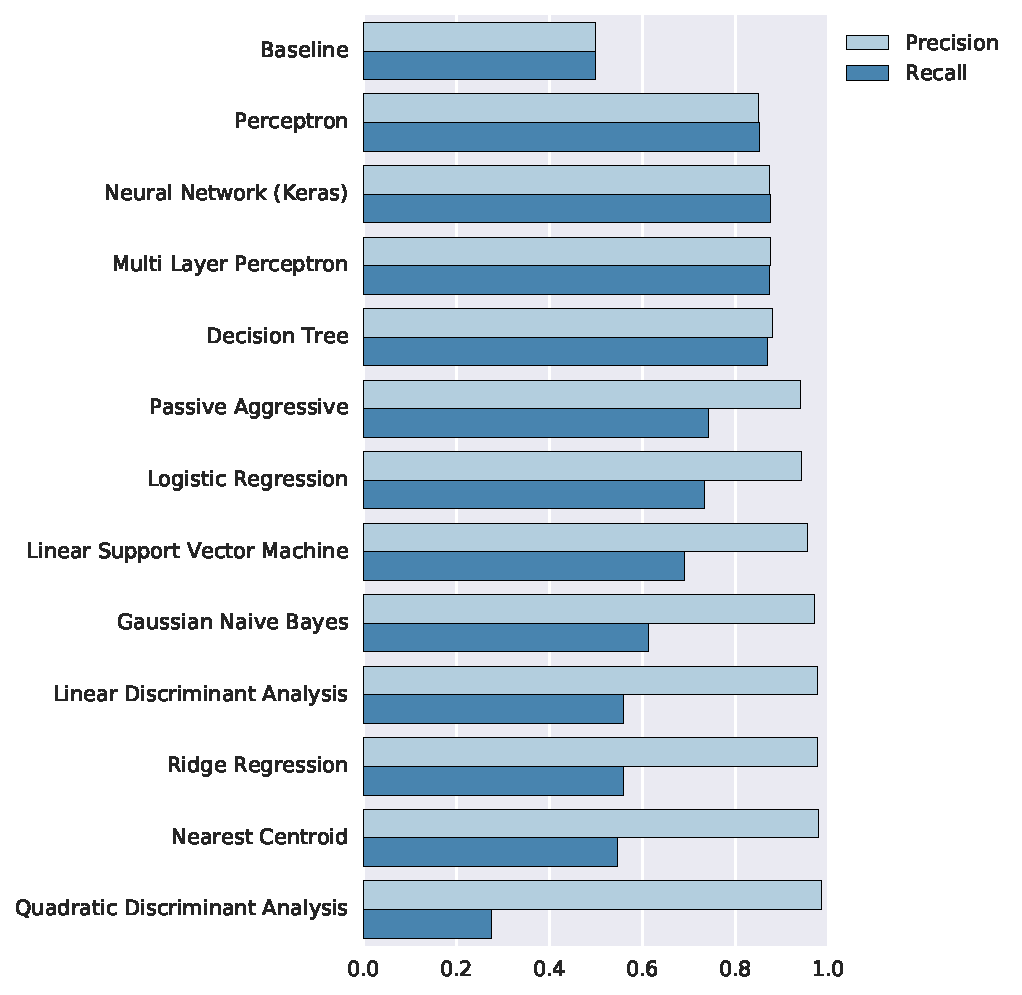
\includegraphics[width=0.95\textwidth]{classifier-comparison2.pdf}
%\caption[Precision and recall scores for the chosen algorithms]{Precision and recall scores for the chosen algorithms, sorted by precision.}\label{fig:classifier_comparison}
%\end{figure}

\begin{figure}[tb]%
\centering
\tikzsetnextfilename{barchart}
\begin{tikzpicture}
  \begin{axis}[
      table/col sep=semicolon,
      xbar=0pt, xmin=0, xmax=1,
      xlabel=Score,
      yticklabels from table={chapter_design/10f-results.csv}{name},
      %yticklabel style={text height=1.5ex},
      ytick=data,
      width=0.6\textwidth,
      y=0.8cm,
      enlarge y limits={abs=0.6},
      bar width=7pt,
      /pgf/number format/fixed,
      axis lines*=left,
      xmajorgrids=true,
      legend entries={Recall, Precision},
      legend style={draw=none},
      reverse legend, area legend,
      legend style={at={(1,1.01)},anchor=south east}
    ]
    \addplot [fill=color1!20!white] table [y expr=-\coordindex, x=recall] {chapter_design/10f-results.csv};
    \addplot [fill=color1!70!white] table [y expr=-\coordindex, x=precision] {chapter_design/10f-results.csv};

  \end{axis}
\end{tikzpicture}
\caption[Precision and recall scores for the chosen algorithms]{Precision and recall scores for the tested algorithms, sorted by precision}\label{fig:classifier_comparison}%
\end{figure}

% \begin{table}[tbp]
% \centering
% \begin{tabular}{@{}lp{.75\textwidth}@{}}
% \toprule
% \textbf{Classifier} & \textbf{Result} \\
% \midrule
% Baseline           &  DummyClassifier()                \\
% Nearest Neighbors  &  KNeighborsClassifier(3)          \\
% Linear SVM         &  SVC(kernel="linear", C=0.025)    \\
% RBF SVM            &  SVC(gamma=2, C=1)                \\
% Gaussian Process   &  GaussianProcessClassifier        \\
% Decision Tree      &  DecisionTreeClassifier           \\
% Random Forest      &  RandomForestClassifier           \\
% Neural Net         &  MLPClassifier, KerasClassifier   \\
% AdaBoost           &  AdaBoostClassifier()             \\
% Naive Bayes        &  GaussianNB()                     \\
% QDA                &  QuadraticDiscriminantAnalysis()  \\
% \bottomrule
% \end{tabular}
% \caption[Classifiers]{Classifiers}%
% \label{tab:classifiers}
% \end{table}

% \subsection{Classifier Parameter Optimization}
% To attempt to further increase the performance of the chosen classifier, we optimize its parameters. The \emph{nearest centroid} implementation in the \emph{scikit-learn} library only has two parameters, so we use grid search to explore possible parameter combinations, as the parameter space is small.

% Searching the parameter space reveals that the default parameters, with a euclidean distance metric, and no feature shrink threshold specified, gives the best performance.


\section[UI]{User Interface}
% Første parameter i [] er tekst i header. {} er i indholdsfortegnelsen.

% Slide med emneoverskrift.
\begin{frame}
  \frametitle{}
  \begin{center}
    {\Huge User Interface}
  \end{center}
\end{frame}
\note{
  \begin{itemize}
		\item Notes...
  \end{itemize}
}

% Normal slide:
\begin{frame}
    \frametitle{Some Example Title}
    \framesubtitle{Some example subtitle}
    \centering
    Some text, content, etc.
\end{frame}
\note{
	\begin{itemize}
    \item Notes here...
	\end{itemize}
}
